\chapter{Low-Resource Data-to-Text Generation}
\label{chap:low-res}


In this chapter, we introduce three approaches for low-resource \ac{d2t} generation based on \acp{plm}. By \emph{low-resource}, we mean using as little data as possible for generating fluent and accurate text. We develop approaches that leverage the general-domain pretraining of \acp{plm} in order to generate texts in domains with thousands, hundreds, or even zero training examples.

The data we focus on are RDF triples from factual knowledge graphs and meaning representations in dialogue systems. The main feature of these kinds of data is that we always want to verbalize the whole input. For larger data, we would need a separate content selection component, but our approaches are generalizable to other kinds of data which fulfill this requirement.

The simplest setting, presented in \autoref{sec:finetuning}, consists of finetuning a pretrained transformer encoder-decoder model. For finetuning the model, we need approximately thousands of in-domain examples. We show that this baseline is powerful, achieving competitive results on a shared task for generating knowledge graph descriptions. On top of that, we show that this approach generalizes to other languages than English, namely Russian.

In \Cref{sec:iterative,sec:pipeline}, we then present approaches which can generate texts with even \emph{more limited amount} of in-domain training examples. Our key idea is to use a \ac{plm} only as a tool for improving text fluency \emph{regardless of the content}, and delegating (possibly crude and basic, but factually correct) verbalization of the content to other, simpler tools. \autoref{sec:iterative} shows an approach using a text-editing model trained on iteratively fusing simple templates, which has a limited vocabulary focused on sentence fusion. The limited vocabulary and training objective pushes the model towards generating factually correct sentences. In \autoref{sec:pipeline}, we also add an ordering and aggregation step for generating more fluent texts. For each of these steps, we can train a \ac{plm} entirely on general-domain operations, reducing the need for in-domain examples to zero.

% \section{Motivation}
% \label{sec:low-res-mot}
\section{Finetuning LMs}
\label{sec:finetuning}

\begin{refbox}
    This section is based on the paper \emph{Train Hard, Finetune Easy: Multilingual Denoising for RDF-to-Text Generation} \cite{kasnerTrainHardFinetune2020}, joint work with Ondřej Dušek, published in the Proceedings of the 3rd International Workshop on Natural Language Generation from the Semantic Web (WebNLG+) at INLG 2020.
\end{refbox}


We introduce a simple approach for generating knowledge graph descriptions. Our approach is based on finetuning a multi-lingual \ac{plm} on linearized graphs and the accompanying human-written descriptions from the WebNLG dataset. In the WebNLG+ Shared Task, our model placed in the first third of the leaderboard for English and first or second for Russian on automatic metrics, and in the best or second-best system cluster on human evaluation.

\subsection{WebNLG+ Shared Task}
\label{sec:webnlgp}
The WebNLG Challenge 2020\footnote{\url{https://synalp.gitlabpages.inria.fr/webnlg-challenge/challenge_2020/}} (WebNLG+; \citealp{ferreira20202020}) was the second edition of the shared task in graph-to-text generation. The task was based on the WebNLG dataset, which contains subgraphs from the DBpedia knowledge graph. Each subgraph is described by a set of RDF triples and accompanied with crowdsourced text descriptions (see \autoref{sec:datasets}). On top of the original challenge \cite{gardentWebNLGChallengeGenerating2017}, WebNLG+ included a separate track of generating texts in Russian, in which we also participated.


\subsection{Problem Formulation}
\label{sec:mbart}
Our input is a set of RDF triples $x \in X$, where each triple $x = (s, p, o)$ describes the relation $p$ between the entities $s$ and $o$ in the knowledge graph. Our target output $Y$ is a fluent and semantically accurate natural language description of $X$.


We formulate the task as \emph{sequence-to-sequence} generation. First, we linearize the input sequence in the default order. We select two arbitrary separator tokens: one to delimit the contituents of the triple and another to delimit individual triples. Using the linearized sequence as an input and the target text, we finetune a pretrained encoder-decoder model using the cross-entropy objective (see \autoref{sec:transformer}). We use the finetuned model to generate the target texts using autoregressive decoding (see Algorithm~\ref{alg:decoding}).

% 


\subsection{Implementation}
\paragraph{Data Preprocessing} We use the provided XML WebNLG data reader\footnote{\url{https://gitlab.com/webnlg/corpus-reader}} to load and linearize the triples. For each triple, we use the \texttt{flat\_triple()} method which converts each triple into the ``\texttt{s $\vert$ p $\vert$ o}'' string, using a pipe (``$\vert$'') as a separator. We use another token not present in the training data (``$\blacktriangleright$'') for delimiting individual triples to avoid extending the model vocabulary.\footnote{Our choice of the separators is arbitrary, as we will adapt the model to account for our separators.
    % Works such as \TODO{cite} or \TODO{cite} show that the choice of separators is not important.
} We linearize the triples in their default order. For the input to the model, we tokenize the data using SentencePiece tokenizer \citep{kudo2018sentencepiece} trained on the training dataset, using a vocabulary of 250,000 subword tokens.

\paragraph{Model}
We use mBART \cite{liuMultilingualDenoisingPretraining2020}, a multilingual \ac{plm} based on BART, a transformer model pretrained on text denoising (see \autoref{sec:plms}).
% In pretraining, the noise function of mBART replaces text spans of arbitrary length with a mask token (35\% of the words in each instance) and permutes the order of sentences. 
The model uses 12 layers for the encoder and 12 layers for the decoder ($\sim$680M parameters), and it is pretrained on the large-scale CC25 corpus extracted from Common Crawl, which contains data in 25 languages \citep{wenzek2020ccnet}.



\paragraph{Training} We finetune the pre-trained \texttt{mbart.CC25} model from the \textsc{fairseq} toolkit \citep{ott2019fairseq} using the default parameters.\footnote{We use dropout 0.3, attention dropout 0.1, and 1024 tokens per batch. We set the initial learning rate to 0.0003 and use polynomial decay with 2500 warmup steps. We train the model using the Adam optimizer \cite{kingma2014adam} with $\beta_1=0.9, \beta_2=0.98$ and $\varepsilon=1e-06$. For the full setup, see \url{https://github.com/facebookresearch/fairseq/tree/main/examples/mbart}.} We change the total number of updates from 40k to 10k to reflect the smaller size of our data. We train a separate version of mBART for each language: $\text{mBART}_{\text{en}}$ on English inputs and English outputs, and $\text{mBART}_{\text{ru}}$ on English inputs and Russian outputs.



\subsection{Results}

\begin{table*}[t]
    \footnotesize
    \centering
    \begin{tabular}{@{}lp{12.7cm}@{}}
        \textbf{input}    & \texttt{Piotr\_Hallmann | weight | 70.308 }  $\blacktriangleright$ \texttt{ Piotr\_Hallmann | birthDate | 1987-08-25} \\
        \textbf{out (en)} & Born on August 25th 1987, Piotr Hallmann has a weight of 70.308.                                                      \\
        \midrule
        \textbf{in}       & \texttt{Ciudad\_Ayala | populationMetro | 1777539}                                                                    \\
        \textbf{out (en)} & The population metro of Ciudad Ayala is 1777539.                                                                      \\
        \midrule
        \textbf{in}       & \texttt{Bakewell\_tart | ingredient | Frangipane}                                                                     \\
        \textbf{out (ru)} & Франжипан - один из ингредиентов тарта Бейквелл.                                                                      \\[0.1cm]
        \textbf{transcr.} & Franzhipan - odin iz ingredientov tarta Bejkvell.                                                                     \\
        \textbf{transl.}  & Frangipane is one of the ingredients of the Bakewell tart.                                                            \\
    \end{tabular}
    \caption{Example outputs from the mBART model(s) finetuned for RDF-to-text generation. (1) The model can work with unseen entities, dates and numbers. (2) The model is quite robust to unseen properties, such as \texttt{populationMetro}. However, the surface form of the property deviates too much from its meaning and the sentence is incorrect. (3) The model trained on Russian targets can use English data to form sentences in Russian, transcribing the entities to Cyrillic.}
    \label{tab:mbart:examples}
\end{table*}

We report on WebNLG automatic and human evaluation results, as well as our own error analysis.

\paragraph{Automatic Metrics}
The results of our approach for English are shown in \autoref{tab:mbart:results-en}, comparing to the baseline.
% \footnote{See \url{https://gerbil-nlg.dice-research.org/gerbil/webnlg2020results} for full results.} 
We can see that our approach beats the baseline in all metrics and places in the first third of the submissions. While it does lose performance on unseen categories, the drop is not as dramatic as for many other competing approaches.

The results for Russian are shown in \autoref{tab:mbart:results-ru}. There were fewer submissions for Russian, and our system not only beats the baseline by a large margin (as did all competing submissions), but it is able to rank first in 2 metrics out of 4 (BLEU, BERTScore) and second in the remaining ones.

\paragraph{Human Evaluation}

The challenge organizers ran a human evaluation campain, where annotators were asked to rate the texts for data coverage, relevance, correctness, text structure and fluency.  Each criterion has been rated with a number in the range from 0 (completely disagree) to 100 (completely agree). The scores were clustered into groups (1-5; 1 being the best) among which there are no statistically significant differences according to the Wilcoxon rank-sum test \citep{wilcoxon1992individual}.

Our systems placed in the top clusters (1 or 2) for both English and Russian. For English, our $\text{mBART}_{\text{en}}$ system ranks first for all the categories in \textit{seen domains}, and first or second in \textit{unseen entities} and \textit{unseen domains}. In total, our English system achieved rank 1 for relevance, correctness and text structure, and rank 2 for data coverage and fluency. For Russian, our $\text{mBART}_{\text{ru}}$ system ranks second for correctness and first in all other categories.


\begin{table*}[t]
    \footnotesize\centering
    \begin{tabular}{llcccccccccc}\toprule
                                     &          & \multicolumn{2}{c}{\bf BLEU} & \multicolumn{2}{c}{\bf METEOR} & \multicolumn{2}{c}{\bf ChrF++} & \multicolumn{2}{c}{\bf BERTScore} & \multicolumn{2}{c}{\bf BLEURT}                                     \\\midrule
        \multirow{2}{*}{All}         & Ours     & 50.34                        & (10)                           & 0.398                          & (8)                               & 0.666                          & (8)  & 0.951 & (8)  & 0.57 & (8)  \\
                                     & Baseline & 40.57                        & (14)                           & 0.373                          & (15)                              & 0.621                          & (15) & 0.943 & (14) & 0.47 & (12) \\\midrule
        \multirow{2}{*}{Seen Cat.}   & Ours     & 59.13                        & (10)                           & 0.422                          & (10)                              & 0.712                          & (9)  & 0.960 & (9)  & 0.58 & (14) \\
                                     & Baseline & 42.95                        & (31)                           & 0.387                          & (27)                              & 0.650                          & (28) & 0.943 & (31) & 0.41 & (31) \\\midrule
        \multirow{2}{*}{Unseen Cat.} & Ours     & 42.24                        & (10)                           & 0.375                          & (13)                              & 0.617                          & (10) & 0.943 & (11) & 0.52 & (10) \\
                                     & Baseline & 37.56                        & (12)                           & 0.357                          & (15)                              & 0.584                          & (15) & 0.940 & (12) & 0.44 & (12) \\\midrule
        \multirow{2}{*}{Unseen Ent.} & Ours     & 51.23                        & (4)                            & 0.406                          & (8)                               & 0.687                          & (7)  & 0.959 & (8)  & 0.63 & (8)  \\
                                     & Baseline & 40.22                        & (17)                           & 0.384                          & (15)                              & 0.648                          & (15) & 0.949 & (13) & 0.55 & (12) \\\bottomrule
    \end{tabular}
    \caption{Results of $\text{mBART}_{\text{en}}$ (all data, seen categories, unseen categories, unseen entities), compared to the baseline. The numbers in brackets show the rank of each model (out of 35 submissions) with respect to the given metric.}
    \label{tab:mbart:results-en}
\end{table*}
\begin{table*}[t]
    \footnotesize\centering
    \begin{tabular}{llcccccccc}\toprule
                 & \multicolumn{2}{c}{\bf BLEU} & \multicolumn{2}{c}{\bf METEOR} & \multicolumn{2}{c}{\bf ChrF++} & \multicolumn{2}{c}{\bf BERTScore}                               \\\midrule
        Ours     & 52.93                        & (1)                            & 0.672                          & (2)                               & 0.677 & (2)  & 0.909 & (1)  \\
        Baseline & 23.53                        & (12)                           & 0.461                          & (12)                              & 0.511 & (12) & 0.836 & (12) \\\bottomrule
    \end{tabular}
    \caption{Results of $\text{mBART}_{\text{ru}}$, compared to the baseline. The numbers in brackets show the rank of each model (out of 12 submissions) if ordered by the given metric.}
    \label{tab:mbart:results-ru}
\end{table*}

\paragraph{Manual Analysis}
To better understand the nature of errors made by our system, we manually inspected a sample of 50 outputs in each language.\footnote{Automatic back-translation to English was used to facilitate understanding of Russian.} We found factual errors in 12 English outputs, mostly concentrated along the unseen categories (\emph{Scientist}, \emph{Movie}, \emph{Musical Record}). The model tends to describe musical works and movies in terms of written works (“written”, “published” etc.), i.e., the closest seen category. There are also several swaps in roles of the entities (e.g., “is to southeast” instead of “has to its southeast”, “follows” instead of “is followed by” etc.).

In a few cases, the model hallucinates a relation not specified in the data (e.g., “born on January 1, 1934 in Istanbul” when a date of birth and current residence is given, not the birthplace) or is not able to infer background knowledge not given on the input (it talks about a dead person in the present tense).
% The swaps in roles and hallucinated relations also occured in Russian; in addition, we found a hallucinated (correct) airport name and a few forgotten ingredients for a dish from a long list. 
Factual errors in Russian were less frequent (9 sentences), which is expected as there are no unseen categories. Moreover, the system shows an impressive performance at translating entity names from the English RDF into Russian.

We further found 10 outputs with suboptimal phrasing in English and 9 in Russian, where the model did not connect properties of the same type in a coordination (e.g., two musical genres for a record) or gave numbers without proper  units (e.g., “runtime of 89.0” or “area of 250493000000.0”).

\paragraph{Discussion}
Our solution benefits from the pretrained representations of the mBART model. Multilingual pretraining allows us to use a single architecture for both English and Russian. However, English and Russian are the two most represented languages in the mBART pre-training corpora (ca. 300 GB of data each) and the performance of our model would probably be lower with low-resource languages.

The performance of our model is also noticeably lower on categories unseen in training, and it is prone to swapping relations of entities or hallucinating relations. Even though the longest examples in the WebNLG dataset fit into the model, the length of the input sequence is still limited and the model does not generalize for inputs of arbitrary size.





\section{Iterative Template Fusion with Text-Editing LMs}
\label{sec:iterative}

\begin{refbox}
    This section is based on the paper \emph{Data-to-Text Generation with Iterative Text Editing} \cite{kasnerDatatoTextGenerationIterative2020}, joint work with Ondřej Dušek, published in the Proceedings of the 13th International Conference on Natural Language Generation (INLG 2020).
\end{refbox}

We present an approach for generating semantically accurate texts from structured data in low-resource settings. Our approach uses a text-editing model (\textsc{LaserTagger}) trained on the task of \emph{sentence fusion}. We first transform individual data items to text using trivial templates, and iteratively improve the resulting text using the \textsc{LaserTagger} model. We evaluate our approach on the WebNLG and E2E datasets, comparing to state-of-the-art approaches. Furthermore, we demonstrate that our task formulation opens up the possibility for zero-shot \ac{d2t} generation by training a model on a general-domain dataset for sentence fusion. The code for the experiments is available on Github.\footnote{\url{https://github.com/kasnerz/d2t_iterative_editing}}


\subsection{Motivation}
\label{sec:text-editing}
Our goal is to improve the semantic accuracy \ac{d2t} generation. Other works have pursued this goal, e.g., by adapting the decoding algorithm \cite{tianStickingFactsConfident2020}, improving robustness of the model by injecting noise in its hidden states \cite{kedzie_good_2019}, or self-training with a natural language understanding model \cite{nieSimpleRecipeReducing2019}. Our approach is inspired by the systems which use a generate-then-rerank approach \citep{dusekSequencetoSequenceGenerationSpoken2016,juraska_deep_2018}, e.g. using a classifier \cite{harkousHaveYourText2020}, to filter incorrect output.

To generate outputs with sufficient semantic accuracy for the filtering step, we take advantage of three facts: (1) we can lexicalize individual data items using trivial templates, (2) concatenating the lexicalizations tends to produce an unnatural sounding but semantically accurate output, and (3) a \ac{plm} trained on improving the output fluency can be used for combining the lexicalizations.

% \textsc{LaserTagger} \cite{malmi2019lasertagger}, which we use in our approach, is a sequence tagging model based on the transformer architecture with BERT \cite{devlinBERTPretrainingDeep2019} as the encoder backbone. Other recent text-editing models without a pre-trained backbone include EditNTS \citep{dong} and Levenshtein Transformer \citep{gu2019levenshtein}.

% Concurrently with our work, \citet{kale2020few} explored using templates for dialogue response generation. %\ODdel{Unlike our work,} 
% They use the sequence-to-sequence T5 model \citep{raffel2019exploring} to generate the output text from scratch instead of iteratively editing the intermediate outputs, which leaves less control over the model.


\subsection{Our Approach}
\label{sec:text-editing-exp}
We focus on data structured as RDF triples.\footnote{Later, we also trivially extend our approach to the data structured as key-value pairs} In our approach, we start from single-triple templates and iteratively fuse them into the resulting text while filtering and reranking the results. We first detail the main components of our system (template extraction, sentence fusion, \ac{plm} scoring) and then give the overall description of the decoding algorithm with filtering and re-ranking.

\begin{figure*}[t]
    \centering
    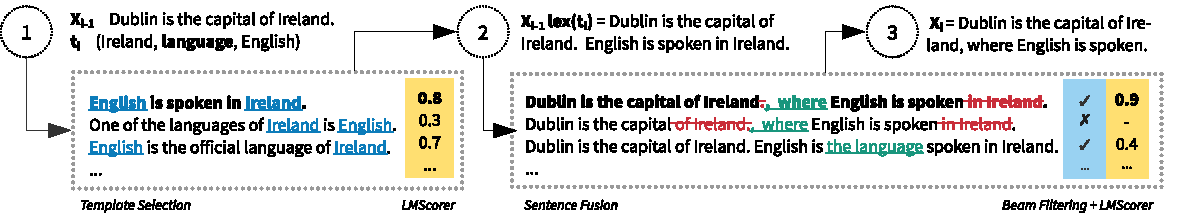
\includegraphics[width=\textwidth]{img/d2t_text_editing}
    \caption{A single iteration of our algorithm for iterative \ac{d2t} generation. In Step 1, the template for the triple is selected and filled. In Step 2, the sentence is fused with the template. In Step 3, the result for the next iteration is selected from the beam by filtering and language model scoring.}\label{fig:iterative:alg}
\end{figure*}



\paragraph{Template Extraction}
We collect a set of templates for each predicate value. There are multiple possibilities for obtaining the templates: we consider (a) handcrafting the template manually for each predicate in the training set, and (b) automatically extracting the template from the lexicalizations of the examples  in the training set. For unseen predicates, we add a single fallback template: \textit{The <predicate> of <subject> is <object>.}


\paragraph{Sentence Fusion}
We train a model for the task of \emph{sentence fusion}, i.e., combining sentences into a coherent text \cite{barzilay2005sentence}.
%We train an independent in-domain sentence fusion model for each dataset. 
To construct the training data, we select pairs $(X, X')$ of examples from the training data consisting of $(k, k+1)$ triples and having $k$ triples in common. This leaves us with an extra triple $t$ present only in $X'$. For each training example, we use the concatenated sequence $X~\mathrm{lex}(t)$ as a source and the sequence $X'$ as a target, where $\mathrm{lex}(t)$ denotes lexicalizing the triple $t$ using an appropriate template. %The operator $\mathrm{lex}(\cdot)$ denotes the lexicalization; the lexicalization of $t$ is obtained by filling the template as described in Section \ref{sec:alg}. 
As a result, the model learns to integrate $X$ and $t$ into a single coherent expression.


\paragraph{PLM Scoring} For re-ranking the text, we use an additional component for computing text fluency, which we refer to as \textsc{LMScorer}.
As described in \autoref{sec:evaluation}, we use perplexity of the text under a a \ac{plm}, computing the score of the output text $Y$ composed of tokens $y_1\ldots y_n$ as a geometric mean of the token conditional probability:
\begin{align}
    \operatorname{score}(Y) = \Bigg( \prod_{i=1}^{n}{P(y_i|y_1 \ldots y_{i-1})} \Bigg)^{\frac{1}{n}}.
\end{align}




\paragraph{Decoding Algorithm}
The input of the algorithm (\autoref{fig:iterative:alg}) is a set of $|T|$ ordered triples. First, we lexicalize the triple $t_0$ to get the output text $X_0$, using the filled template with the best score from \textsc{LMScorer}.
% This promotes templates which sound more natural for particular values.
In each of the following steps $i=1\ldots |T|-1$, we lexicalize the triple $t_i$ and concatenate it with $X_{i-1}$.  For improving the fluency of the text, we use the sentence fusion model with beam search to produce $k$ hypotheses. We filter and re-rank the hypotheses, getting $X_{i}$ (see the next paragraph), and proceed to the next step. The output of the algorithm is the text $X_{|T|}$ from the final step.


\paragraph{Filtering and Re-ranking} In each decoding step, we remove hypotheses in the beam missing any entity from the input data using a simple heuristic based on string matching. Next, we rescore the remaining hypotheses in the beam with \textsc{LMScorer} and set the hypothesis with the best score as $X_{i}$. In case there are no sentences left in the beam after the filtering step, we let $X_{i}$ be the text in which the lexicalized $t_i$ is appended after $X_{i-1}$ without sentence fusion.

%For the E2E dataset, we first try to find a pair of predicates for which there is a template extracted from the data, and only use the handcrafted templates for the single predicates in the subsequent steps. 
%The final beam filtering step is a simple heuristic, checking if all entities from the input triples are present in the output.


\subsection{Experiments}
\paragraph{Datasets}





\begin{table}[t]
    \centering\footnotesize
    \begin{tabular}{llll}
        \textbf{dataset} & \textbf{method} & \textbf{predicate}          & \textbf{example templates }                                                                \\\midrule
        WebNLG           & extracted       & \texttt{foundedBy}          & \textit{$o$ was the founder of $s$.} | \textit{$s$ was founded by $o$.}                    \\
        E2E              & extracted       & \texttt{area}+\texttt{food} & \textit{$s$ offers $o_2$ cuisine in the $o_1$.} | \textit{$s$ in $o_1$ serves $o_2$ food.} \\
        E2E              & manual          & \texttt{near}               & \textit{$s$ is located near $o$.}                 | \textit{$o$ is close to $s$.}
    \end{tabular}
    \caption{Examples of templates we used in our experiments. The templates for the single predicates in the WebNLG dataset and the pairs of predicates in the E2E dataset are extracted automatically from the training data; the templates for the single predicates in E2E are created manually.}
    \label{tab:iterative:templates_ex}
\end{table}


\paragraph{Template extraction} For WebNLG, we extract the initial templates from the training data from examples containing only a \textit{single} triple. In the E2E dataset, there are no such examples; therefore our solution is twofold: we extract the templates for \textit{pairs} of predicates, using them as a starting point for the algorithm in order to leverage the lexical variability in the data (manually filtering out the templates with semantic noise), and we also create a small set of templates for each \textit{single} predicate manually, using them in the subsequent steps of the algorithm (this is possible due to the low variability of the predicates in the dataset).\footnote{In the E2E dataset, the data is in the form of key-value slots. We transform the data to RDF triples by using the name of the restaurant as a \textit{subject} and the rest of the slots as \textit{predicate} and \textit{object}. This creates \textit{n-1} triples for \textit{n} slots.} See \autoref{tab:iterative:templates_ex} for examples of templates we used in our experiments.

\paragraph{Sentence Fusion Model} We base our sentence fusion model on \textsc{LaserTagger} \cite{malmi2019lasertagger}. \textsc{LaserTagger} is a sequence generation model which generates outputs by tagging inputs with edit operations: \texttt{KEEP} a token, \texttt{DELETE} a token, and \texttt{ADD} a phrase before the token. In tasks where the output highly overlaps with the input, such as sentence fusion, \textsc{LaserTagger} is able to achieve performance comparable to state-of-the-art models with faster inference times and less training data.

\paragraph{Limited Vocabulary} An important feature of \textsc{LaserTagger} is the limited size of its vocabulary, which consists of $l$ most frequent (possibly multi-token) phrases used to transform inputs to outputs in the training data. After the vocabulary is precomputed, all infeasible examples in the training data are filtered out. At the cost of limiting the number of training examples, this filtering makes the training data cleaner by removing outliers. The limited vocabulary also makes the model less prone to common neural model errors such as hallucination, which allows us to control the semantic accuracy to a great extent using only simple heuristics and language model rescoring.

\paragraph{LMScorer} In our case,  \textsc{LMScorer} is a pre-trained GPT-2 language model \citep{radford2019language} from the Transformers repository\footnote{\url{https://github.com/huggingface/transformers}} \citep{Wolf2019HuggingFacesTS} wrapped in the \textit{lm-scorer}\footnote{\url{https://github.com/simonepri/lm-scorer}} package.





\begin{table*}[t]% \begin{adjustbox}{max width=\textwidth}
    \centering\footnotesize
    \begin{tabular}{lcccc<{\hspace{2mm}}c>{\hspace{2mm}}cccc} \toprule
                         & \multicolumn{4}{c}{\bf WebNLG} &            & \multicolumn{4}{c}{\bf E2E}                                                                                                                                                                          \\
        \cmidrule{2-5} \cmidrule{7-10}
                         & {\it BLEU}                     & {\it NIST} & \hspace{-1mm}{\it METEOR}\hspace{-1mm} & \hspace{-1mm}{\it ROUGE$_L$}\hspace{-1mm} &  & {\it BLEU} & {\it NIST} & \hspace{-1mm}{\it METEOR}\hspace{-1mm} & \hspace{-1mm}{\it ROUGE$_L$}\hspace{-1mm} \\
        {\bf baseline}   & 0.277                          & 6.328      & 0.379                                  & 0.524                                     &  & 0.207      & 3.679      & 0.334                                  & 0.401                                     \\
        {\bf zero-shot } & 0.288                          & 6.677      & 0.385                                  & 0.530                                     &  & 0.220      & 3.941      & 0.340                                  & 0.408                                     \\
        {\bf w/fusion }  & 0.353                          & 7.923      & 0.386                                  & 0.555                                     &  & 0.252      & 4.460      & 0.338                                  & 0.436                                     \\
        {\bf SFC }       & 0.524                          & -          & 0.424                                  & 0.660                                     &  & 0.436      & -          & 0.390                                  & 0.575                                     \\
        {\bf T5 }        & 0.571                          & -          & 0.440                                  & -                                         &  & -          & -          & -                                      & -                                         \\ \bottomrule
    \end{tabular}
    \caption{Results of automatic metrics on the WebNLG and E2E test sets. The comparison is made with the results from the papers on the Semantic Fidelity Classifier (SFC; \citealp{harkousHaveYourText2020}) and the finetuned T5 model (T5; \citealp{kaleTexttoTextPreTrainingDatatoText2020}), state-of-the-art approaches at that time.}
    \label{tab:results}
    % \end{adjustbox}
\end{table*}




\subsection{Setup}
As a \emph{baseline}, we generate the best templates according to \textsc{LMScorer} without applying the sentence fusion (i.e.\ always using the fallback).

For the \emph{sentence fusion} experiments, we use \textsc{LaserTagger} with the autoregressive decoder with a beam of size 10. We use all reference lexicalizations and the vocabulary size $V=100$, following our preliminary experiments, which showed that filtering the references only by limiting the vocabulary size brings the best results (see Supplementary for details). We finetune the model for 10,000 updates with batch size 32 and learning rate $2 \times 10^{-5}$.
For the beam filtering heuristic, we check for the presence of entities by simple string matching in WebNLG; for the E2E dataset, we use a set of regular expressions from TGen\footnote{\url{https://github.com/UFAL-DSG/tgen}} \citep{dusek_semantic_2019}. We do not use any pre-ordering steps for the triples and process them in the default order.

Additionally, we conduct a \textit{zero-shot domain adaptation} experiment. We train the sentence fusion model with the same setup, but instead of the in-domain datasets, we use a subset of the balanced-Wikipedia portion of the \textsc{DiscoFuse} dataset. In particular, we use the discourse types which frequently occur in our datasets, filtering the discourse types which are not relevant for our use-case. See Supplementary for the full listing of the selected types.


% \vspace{-3mm}

\begin{table*}[t] \footnotesize
    \begin{tabular}{l p{12cm}}
        \textbf{Triples}   & \textit{(Albert Jennings Fountain, deathPlace, New Mexico Territory); (Albert Jennings Fountain, birthPlace, New York City); (Albert Jennings Fountain, birthPlace, Staten Island)} \\ \midrule
        \textbf{Step \#0}  & Albert Jennings Fountain died in New Mexico Territory.                                                                                                                              \\
        \textbf{Step \#1}  & Albert Jennings Fountain, who died in New Mexico Territory, was born in \greenund{New York City}.                                                                                   \\
        \textbf{Step \#2}  & Albert Jennings Fountain, who died in New Mexico Territory, was born in New York City, \greenund{Staten Island}.                                                                    \\ \midrule
        \textbf{Reference} & Albert Jennings Fountain was born in Staten Island, New York City and died in the New Mexico Territory.
    \end{tabular}
    \caption{An example of correct behavior of the algorithm on the WebNLG dataset. Newly added entities are underlined, the output from Step \#2 is the output text.}\label{tab:ex0}
\end{table*}


\section{Pipelined Text-Based Operations with Pretrained LMs}
\label{sec:pipeline}
\subsection{Pipeline Operations}
\label{sec:pipeline-ops}
\subsection{Experiments}
\label{sec:pipeline-exp}
